\section{Introduction}
Photo-realistic image generation has a long tradition in computer graphics and the topic is still far from being exhausted. Among other rendering techniques, physically based rendering plays a key role in modern graphics applications. Ray tracing can be used as such a rendering technique by simulating how light travels through a scene, creating physically plausible images in the process. Consequently, this method has long been a staple in offline rendering, where relatively long rendering times can be tolerated. In real-time applications, however, a rapid rate of images is required to achieve fluent motion. Video games require a frame rate of at least 30 frames per second (FPS), but modern titles tend to target faster rates of 60 FPS and above. Ray tracing is a very computation heavy task and even interactive rates, starting at 6 FPS, can be a daunting task. 

As a result, rasterization has dominated real-time rendering and, until fairly recently, has been seen as the sole viable approach. Rasterization takes a divide and conquer approach by dividing a scene into a mesh of basic geometric shapes (e.g. triangles). 
\begin{figure}
    \centering
    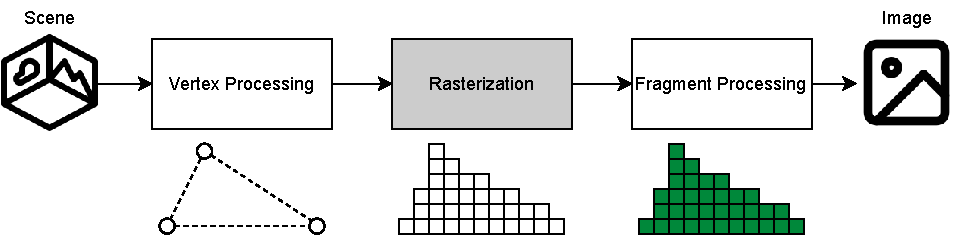
\includegraphics[width=400pt]{images/rasterization_pipeline.pdf}
    \caption{Simplified Rasterization Pipeline.}
    \label{fig:raster_pipeline}
\end{figure}
These are sent to a rendering pipeline (figure \ref{fig:raster_pipeline}), where each is processed individually. First, vertices are transformed and projected into screen space. The results are then fed to a rasterizer, which performs spatial sampling to determine which pixels are occupied by given primitive. These pixels, often referred to as fragments, are then assigned a color derived from a number of operations. A Z-buffer algorithm is used to determine which fragments are occluded and any visible fragment is written to a frame buffer. This process is highly parallel and can be executed very efficiently on conventional GPUs. One drawback of that parallelism is, that only a single primitive is considered at a time. Effects like shadows, reflections and refractions, however, can only be achieved by taking multiple primitives into account. In practice, complex methods are used to approximate such effects.

By emulating the basic concepts of vision, ray tracing achieves the same effects much simpler and more natural. In reality, objects are perceived after a light ray hits said object and then bounces into the eye. This concept is recreated in ray tracing, only in the reversed way. For each pixel, a ray is cast from the eye point and bounces around the scene until a termination criteria is met. Several billion rays are necessary, to converge towards a sufficient solution of that approach, hence the high computational effort. 

In recent years, however, these limitations have been overcome and real-time ray tracing has been enabled and opened up to a consumer market, especially through the use of special-purpose hardware. Such hardware\cite{nvidia2017turing} is built in a way that accelerates basic ray tracing operations while also facilitating other methods essential to the process, most importantly more advanced denoising techniques. While this technology is undoubtedly a leap in the right direction, performance can still lack at times and additional software optimizations are necessary to support increasingly complex scenes. Additionally, such optimizations could decrease the power consumption of graphic cards by decreasing the number of computations necessary and could be utilized by conventional ray tracing frameworks as well. This thesis continues on previous findings and aims to identify more areas of improvement and then optimize them.
\\\\
In particular, this thesis provides a self-contained overview over the basics of real-time ray tracing (section \ref{path_tracing_basics}) as well as a broader outline over some related topics, which are important in that context. Acceleration data structures are explored in more detail (section \ref{acceleration_structure_basics}) and a construction method based on the approach of \acrfull{phr}\cite{hendrich_parallel_2017} is presented as a state-of-the art algorithm (section \ref{phr}). The viability of progressive hierarchical refinement in interactive ray tracing is then evaluated based on a CPU path tracer written from scratch in the programming language Go. Key implementation decisions of said path tracer are explained in more detail (section \ref{path_tracer}), which might be particularly helpful as a starting point for further research. A novel approach for optimizing the build-trace trade-off of PHR is proposed(section \ref{parameters}), evaluated (section \ref{results}). Finally, the thesis is concluded by discussing all findings (section \ref{discussion}) and identifying future work (section \ref{conclusion})
\cleardoublepage